\section{Results}\label{sec:results}

\subsection{First, make sure the database is what saturates}\label{sec:apifirst}
Our first two attempts did not measure the database. With 8 API workers $\times$ 8 pooled connections the publish
curve flattened at $\approx$300 posts/s, but the database had only 3.5--5 busy backends and a home-feed
\emph{read}, which barely touches the database, was capped at the same $\approx$380 requests/s: the API's
connection pool was the bottleneck (each request holds a connection for a 75~ms round trip). Raising the pool to
16$\times$12 moved the plateau to $\approx$460 posts/s with the same symptom. With the final setting (6 workers
$\times$ 32 connections per shard; at most 192 client connections per project, below the Supabase pooler's 200)
a feed read reaches 1{,}571 requests/s and a like 1{,}330 requests/s through the same API with the database almost idle,
while publish saturates at $\approx$574 posts/s. The request path can therefore carry at least 2.7$\times$ the
publish throughput we report, so the publish plateau below is a database limit. The superseded runs are kept in
\texttt{m6/results-run1-apipool/} and \texttt{m6/results-run2-api16x12/}.

\subsection{Before sharding: writes are the bottleneck}\label{sec:bottleneck}

\begin{figure}[H]\centering
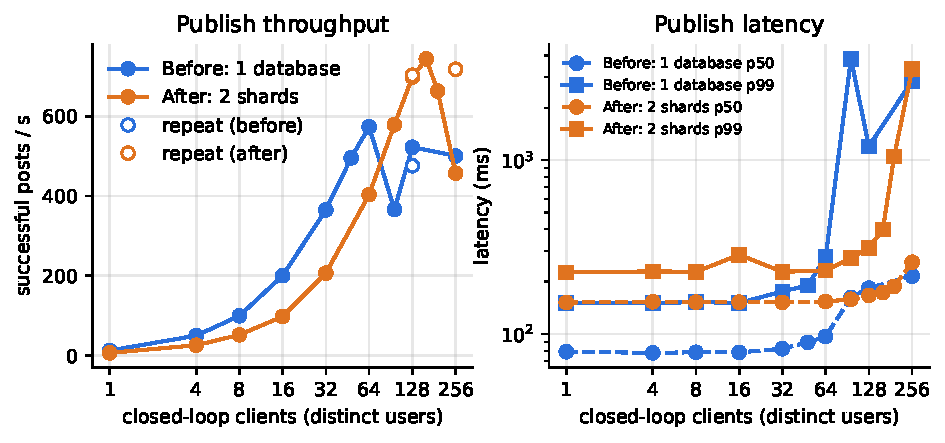
\includegraphics[width=\linewidth]{figures/post_throughput_latency.pdf}
\caption{Publish staircase, one database (blue) vs.\ two shards (orange). Hollow points are repeated stages.
Each point is a 30~s closed-loop stage with distinct users; zero errors in every stage.}
\label{fig:tput}
\end{figure}

\paragraph{Throughput and latency.} With one database, publish throughput grows linearly up to 32 clients
(365 posts/s, p99 176~ms), peaks at \textbf{574 posts/s at 64 clients} (25{,}600 rows inserted/s, 10.8~MB/s of WAL),
and then \emph{falls} as more writers are added: 522 posts/s at 128 clients and 501 at 256, while p99 rises from
276~ms to 1.2~s and 2.9~s. The 96-client stage was unstable (366 posts/s, p99 3.8~s). The repeated 128-client stage
gave 476 posts/s, 9\% below the first run; the shared Nano instance is noisy once it is overloaded. More clients past
the knee only add queueing; Little's law holds in every stage (Table~\ref{tab:little}).

\paragraph{Where the time goes inside the database.} The 1~Hz \texttt{pg\_stat\_activity} samples
(Figure~\ref{fig:waits}) show the number of busy backends rising from 1.5 (16 clients) to 14--15.6 (64 clients and
above), which is the Supabase pooler's 15 server connections for a Nano project. On a 2-vCPU machine, 7--10 of them are
runnable on CPU, and 3--4 wait on \texttt{LWLock:WALWrite} / \texttt{IO:WalSync}, i.e.\ for their commit record to
reach disk, plus 1--3 on buffer-content and relation-extension locks. The same statement got slower as load rose:
the mean execution time of \texttt{publish\_post()} went from 3.4~ms (16 clients) to 7.0, 11.6, 16.8 and 22--24~ms
(32, 48, 64, $\ge$128 clients). The work per post did not change (46 rows, one commit), so this 7$\times$ slowdown is contention.

\begin{figure}[H]\centering
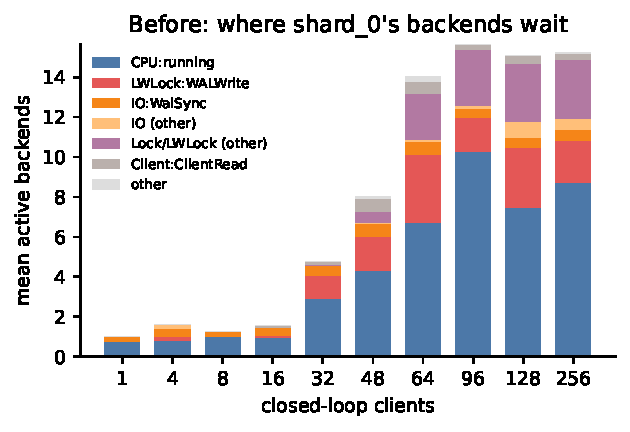
\includegraphics[width=0.56\linewidth]{figures/waits_before.pdf}\hfill
\begin{minipage}[b]{0.42\linewidth}\small
\captionof{figure}{One database: mean number of active backends by wait event (1~Hz samples). Blue = on CPU;
red/orange = waiting for the WAL to be written and flushed (commit).}\label{fig:waits}
\vspace{6mm}
\end{minipage}
\end{figure}

\paragraph{The host.} Supabase's metrics endpoint refreshes about every 60~s, so we logged it continuously and plot
it against the stage windows (Figure~\ref{fig:hostS1}). During the saturated publish stages (64--256 clients) the database VM spent
34--61\% of its CPU in user+system time and another 18--44\% in \textbf{iowait}; busy+iowait stayed at 73--79\%,
leaving about 20\% idle, and it wrote 16--21~MB/s to disk. The two cores are either computing inserts and index updates or waiting for the disk.

\begin{figure}[H]\centering
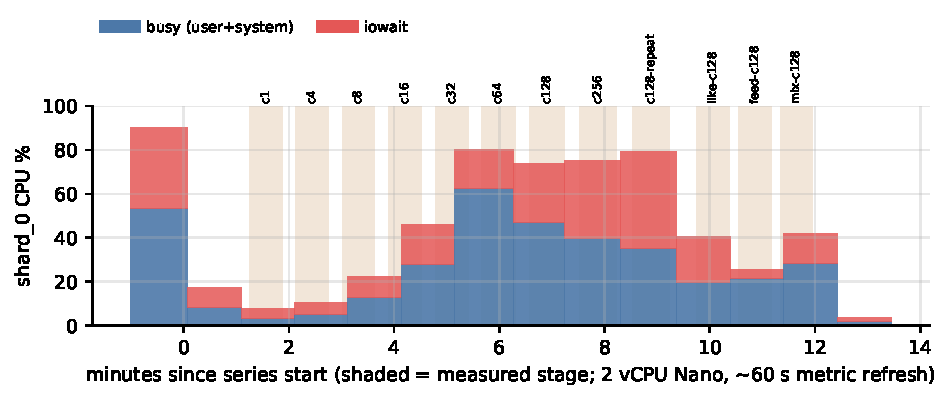
\includegraphics[width=\linewidth]{figures/host_cpu_S1.pdf}
\caption{One database: shard\_0 VM CPU per metrics refresh (blue = user+system, red = iowait). Shaded bands are the measured stages.}
\label{fig:hostS1}
\end{figure}

\paragraph{Step 1 query.} The handout query (statements starting with INSERT/UPDATE/DELETE) returns no rows for
Campus Pulse, because every busy write runs inside a stored procedure called with \texttt{SELECT}. Over all
statements, \texttt{publish\_post()} accounts for 98.8\% of the execution time of the top ten statements and wrote
1.53~GB of WAL during the one-database staircase:

\begin{center}\scriptsize
\begin{tabular}{@{}llrrrr@{}}
\toprule
Shard & Statement (\texttt{pg\_stat\_statements}, after the S1 staircase) & Calls & Total ms & Mean ms & WAL MB \\
\midrule
\tabinput{tables/step1_S1.tex}
\bottomrule
\end{tabular}
\end{center}

\noindent\textbf{Conclusion for Step 1:} writes are the bottleneck. The top statement is the write path, the
database runs out of connections, CPU and commit bandwidth, more clients make throughput worse, and the cheaper fixes
from slide~25 are already in place (one stored-procedure call per post, no counter row, no unused index). The next
cheapest fix would be a bigger compute plan; the assignment asks us to shard.

\subsection{After sharding: the same staircase on two databases}

\begin{figure}[H]\centering
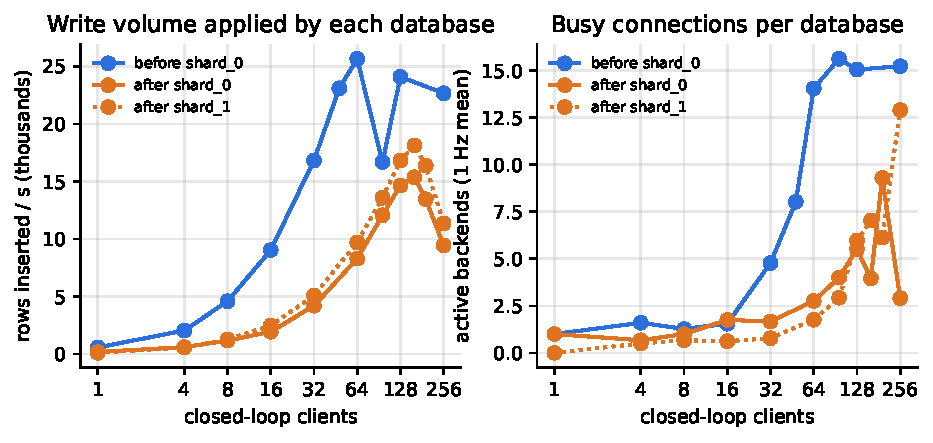
\includegraphics[width=\linewidth]{figures/db_per_shard.pdf}
\caption{Rows inserted per second and busy backends, per database. After sharding, each database applies about half
of the rows, and neither database reaches the 15-backend ceiling at the throughputs where the single database is saturated.}
\label{fig:pershard}
\end{figure}

\paragraph{Capacity.} With two shards, publish peaks at \textbf{744 posts/s at 160 clients} (p99 398~ms), and stays at
698--744 posts/s from 128 to 160 clients with p99 $\le$ 400~ms. The one-database peak was 574 posts/s with p99 276~ms. The
peak is 1.30$\times$ higher, and over the saturated region the median is 700 vs.\ 501 posts/s (1.40$\times$). At 192 and 256 clients the
two-shard system also overloads (663 and 457/718 posts/s, p99 up to 3.3~s; the two 256-client runs differ by 57\%).

\paragraph{Load per database.} Compare stages with the same throughput: one database at 64 clients (574 posts/s) and two
shards at 96 clients (579 posts/s). Each shard inserted 12.1k and 13.6k rows/s instead of 25.6k, had 4.0 and 2.9 busy
backends instead of 14.1, and ran \texttt{publish\_post()} in 3.5~ms instead of 16.8~ms. Halving the rows per database
removed most of the contention, so each shard is far below its own saturation point while carrying the same user load.

\paragraph{Latency at low load got worse.} At 1--64 clients, two shards deliver about half the throughput of one database
at the same concurrency (403 vs.\ 574 posts/s at 64 clients), and p50 rises from 78 to 153~ms. The cause is the
cross-shard copy: a post now commits on the author's shard and then writes follower copies on the other shard,
written second as the lecture requires, so one click costs two sequential 75~ms round trips. Closed-loop throughput
at fixed concurrency is $c/R$, so it halves until the databases saturate.

\begin{figure}[H]\centering
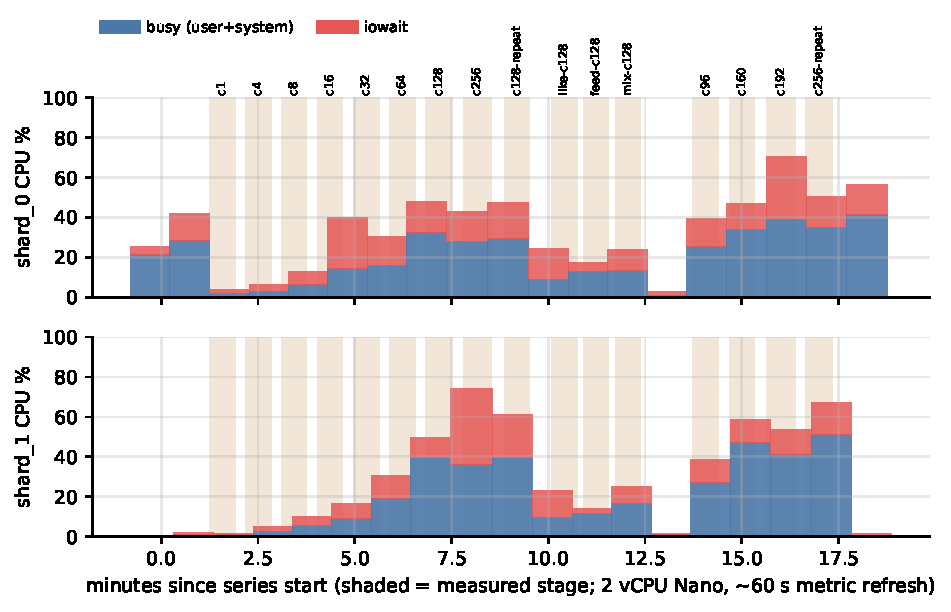
\includegraphics[width=\linewidth]{figures/host_cpu_S2.pdf}
\caption{Two shards: VM CPU of both databases. In the 128-client stages both are around 45--50\% busy+iowait; the
first 256-client stage drove shard\_1 to 74\% (iowait 38\%) while shard\_0 stayed near 43\%.}
\label{fig:hostS2}
\end{figure}

\paragraph{The busiest shard decides.} shard\_1 owns 219 of the 400 users (55\%; buckets are hashed, so the split is
close but not exact) and therefore receives 24 rows per post vs.\ 21 on shard\_0. In the first 256-client stage shard\_1's
\texttt{publish\_post()} took 22.9~ms and it had 12.9 busy backends, while shard\_0 had 2.9. Every post waits for both
shards, so the slower shard set the throughput (457 posts/s). This is lecture slide~15: capacity is the busiest
shard.

\paragraph{Other workloads (128 clients).}
\begin{center}\footnotesize
\begin{tabular}{@{}lrrrrl@{}}
\toprule
Workload & 1 DB req/s & 2 shards req/s & Change & p99 (1 DB $\to$ 2) & Note \\
\midrule
Like (1-row insert) & 1{,}330 & 1{,}609 & +21\% & 188 $\to$ 148 ms & commit waits gone; API ceiling \\
Home-feed read & 1{,}571 & 1{,}636 & +4\% & 149 $\to$ 148 ms & DB nearly idle in both \\
70/20/10 mix & 1{,}553 & 1{,}484 & $-$4\% & 150 $\to$ 160 ms & posts pay a 2nd round trip \\
\bottomrule
\end{tabular}
\end{center}
Reads did not get faster, and the lecture says they should not: sharding adds write capacity. The home feed remained a
one-shard query because its rows are copies on the reader's shard.

\subsection{Correctness checks (lecture slide 41)}
\begin{center}\small
\begin{tabular}{@{}lll@{}}
\toprule
Check & Result (two shards) & Expected \\
\midrule
Users per shard (\texttt{count(*)} on each) & shard\_0: 181, shard\_1: 219 & close, not identical \\
Users per shard via directory $\bowtie$ bucket\_map & shard\_0: 181, shard\_1: 219 & same as above \\
Rows on the wrong shard & 0 and 0 & 0 \\
\texttt{bucket\_map} & 32 / 32 buckets & 32 / 32 \\
Bad insert (bucket 37) on shard\_0 & rejected: violates \texttt{users\_belong\_here} & rejected \\
Python \texttt{shard\_bucket} vs.\ SQL, 2{,}000 ids & identical on both shards & identical \\
\bottomrule
\end{tabular}
\end{center}

\subsection{All stages}
Per-stage results; for two shards, per-database columns are given as shard\_0 / shard\_1. ``Exec'' = seconds of
statement execution per second (from \texttt{pg\_stat\_statements}); ``Busy'' = mean active backends; API CPU in \% of one core.
\begin{center}\scriptsize\setlength{\tabcolsep}{3pt}
\resizebox{\linewidth}{!}{%
\begin{tabular}{@{}lrrrrrrrrllll r@{}}
\toprule
Workload & $c$ & Requests & OK/s & p50 & p95 & p99 & max & Err & Rows/s (k) & Exec s/s & Busy & WAL MB/s & API \\
\midrule
\multicolumn{14}{@{}l}{\textbf{Before: one database (S1)}} \\
\tabinput{tables/stages_S1.tex}
\midrule
\multicolumn{14}{@{}l}{\textbf{After: two shards (S2)}} \\
\tabinput{tables/stages_S2.tex}
\bottomrule
\end{tabular}}
\end{center}

\begin{table}[H]\centering\small
\caption{Little's law check: in-flight requests $L = X\cdot R$ match the closed-loop client count $c$.}\label{tab:little}
\begin{tabular}{@{}rlrrrr@{}}
\toprule
Shards & Workload & $c$ & $X$ (req/s) & $R$ mean (ms) & $L = X R$ \\
\midrule
\tabinput{tables/little.tex}
\bottomrule
\end{tabular}
\end{table}
